\documentclass[uplatex, dvipdfmx]{jsarticle}


\usepackage{tcolorbox}
\usepackage{color}
\usepackage{listings, plistings}

%% ノート/latexメモ
%% http://pepper.is.sci.toho-u.ac.jp/pepper/index.php?%A5%CE%A1%BC%A5%C8%2Flatex%A5%E1%A5%E2

%% JavaScriptの設定
%% https://e8l.hatenablog.com/entry/2015/11/29/232800
\lstdefinelanguage{javascript}{
  morekeywords = [1]{ %keywords
    await, break, case, catch, class, const, continue, debugger, default, delete, 
    do, else, enum, export, extends, finally, for, function, function*, if, implements, import, in, 
    instanceof, interface, let, new, package, private, protected, public, return, static, super,
    switch, this, throw, try, typeof, var, void, while, with, yield, yield*
  },
  morekeywords = [2]{ %literal
    false, Infinity, NaN, null, true, undefined
  },
  morekeywords = [3] { %Classes
    Array, ArrayBuffer, Boolean, DataView, Date, Error, EvalError, Float32Array, Float64Array,
    Function, Generator, GeneratorFunction, Int16Array, Int32Array, Int8Array, InternalError,
    JSON, Map, Math, Number, Object, Promise, Proxy, RangeError, ReferenceError, Reflect,
    RegExp, Set, String, Symbol, SyntaxError, TypeError, URIError, Uint16Array, Uint32Array,
    Uint8Array, Uint8ClampedArray, WeakMap, WeakSet
  },
  morecomment = [l]{//},
  morecomment = [s]{/*}{*/},
  morestring = [b]{"},
  morestring = [b]{'},
  alsodigit = {-},
  sensitive = true
}

%% 修正時刻: Tue 2022/03/15 10:04:41


% Java
\lstset{% 
  frame=single,
  backgroundcolor={\color[gray]{.9}},
  stringstyle={\ttfamily \color[rgb]{0,0,1}},
  commentstyle={\itshape \color[cmyk]{1,0,1,0}},
  identifierstyle={\ttfamily}, 
  keywordstyle={\ttfamily \color[cmyk]{0,1,0,0}},
  basicstyle={\ttfamily},
  breaklines=true,
  xleftmargin=0zw,
  xrightmargin=0zw,
  framerule=.2pt,
  columns=[l]{fullflexible},
  numbers=left,
  stepnumber=1,
  numberstyle={\scriptsize},
  numbersep=1em,
  language={Java},
  lineskip=-0.5zw,
  morecomment={[s][{\color[cmyk]{1,0,0,0}}]{/**}{*/}},
  keepspaces=true,         % 空白の連続をそのままで
  showstringspaces=false,  % 空白字をOFF
}
%\usepackage[dvipdfmx]{graphicx}
\usepackage{url}
\usepackage[dvipdfmx]{hyperref}
\usepackage{amsmath, amssymb}
\usepackage{itembkbx}
\usepackage{eclbkbox}	% required for `\breakbox' (yatex added)
\usepackage{enumerate}
\usepackage[default]{cantarell}
\usepackage[T1]{fontenc}
\fboxrule=0.5pt
\parindent=1em
\definecolor{mygrey}{rgb}{0.97, 0.97, 0.97}

\makeatletter
\def\verbatim@font{\normalfont
\let\do\do@noligs
\verbatim@nolig@list}
\makeatother

\begin{document}

%\anaumeと入力すると穴埋め解答欄が作れるようにしてる。\anaumesmallで小さめの穴埋めになる。
\newcounter{mycounter} % カウンターを作る
\setcounter{mycounter}{0} % カウンターを初期化
\newcommand{\anaume}[1][]{\refstepcounter{mycounter}{#1}{\boxed{\phantom{aa}\textnormal{\themycounter}\phantom{aa}}}} %穴埋め問題の空欄作ってる。
\newcommand{\anaumesmall}[1][]{\refstepcounter{mycounter}{#1}{\boxed{\tiny{\phantom{a}\themycounter \phantom{a}}}}}%小さい版作ってる。色々改造できる。

%% 修正時刻: Tue 2022/03/15 10:04:411


\section{MySQLにログインする}

\subsection{root(管理者)でログインする}

データベースを利用するためには、まず、そのデータベースを管理している人
(管理者)から、アカウント(ユーザー名とパスワード)を発行してもらわなくては
ならない。

そして、通常は1つのデータベースが与えられ、そのデータベースの中に
複数のテーブル(表)を作成していくことになる。

しかし、ここでは 管理者のままで MySQLデータベースを操作していくことにする。
そして、操作に慣れたら、一般ユーザーを作成し、一般ユーザーとして
データベースを操作していくことにする。

\vspace{6mm}
\textgt{管理者(root) でのログイン}

\begin{lstlisting}[numbers=none]
mysql> mysql -u root -p
Enter password: ****  
\end{lstlisting}

あるいは、一行で書ける。この場合、パスワードが表示される。
パスワードは -p のあと、空白をはさまずに続けて書く。

 \fbox{mysql$>$ mysql -u root -proot}
 \footnote{\textsf{mysql} コマンドは、
 ``C:\yen MAMP\yen bin\yen mysql\yen bin'' の
 中の ``mysql.exe'' のことである。
 このフォルダには、他にも ``mysqldump.exe'' など
 いろいろなコマンドが置かれている。}


\section{データベースを設計する}

\subsection{扱うデータ}

以下のようなデータを扱うこととする。

\vspace{3mm}
 \begin{tabular}{|c|} \hline
  菅原文太 \\
  40歳 \\
  1933年生まれ \\
  総務部 \\ \hline
 \end{tabular}
 \quad
 \begin{tabular}{|c|} \hline
  千葉真一 \\
  34歳 \\
  1939年生まれ \\
  営業部 \\ \hline
 \end{tabular}
 \quad
 \begin{tabular}{|c|} \hline
  北大路欣也 \\
  30歳 \\
  1943年生まれ \\
  経理部 \\ \hline
 \end{tabular}
 \quad
 \begin{tabular}{|c|} \hline
  梶芽衣子 \\
  26歳 \\
  1947年生まれ \\
  営業部 \\ \hline
 \end{tabular}
\vspace{3mm}

あなたがプログラマで、上のような社員名簿アプリを作成することになったとする。
PHP か Java でアプリを作成することになる。クライアントの会社の総務部がこの
アプリを使うことになる。そのアプリには社員の登録画面、一覧画面、編集画面、
削除画面などがあるだろう。そういった画面と処理をあなたは作らなければならない。

そのときに、データを保存するしくみとして、データベースを使うことになる。
かりに PHP でプログラミングするならば、PHPという言語を使って
データベースを操作することになる。

\subsection{どのような表をつくるか?}

データベースは表の形でイメージすることができる。
しかし、上記のデータを見て、それをそのまま表にしてはいけない。

\vspace{3mm}
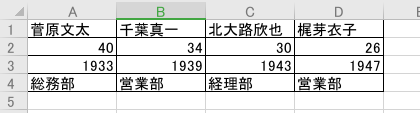
\includegraphics[width=10cm]{img/table01.png}
\vspace{3mm}

この表は、1件のデータが縦に配置されて、それが人数分横に続いている。これは良くない。

次の表のように、1件のデータを横に配置する。

\vspace{3mm}
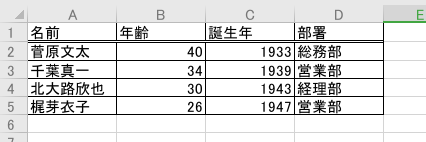
\includegraphics[width=10cm]{img/table02.png}
\vspace{3mm}

そして、縦には同じ種類のデータが並ぶ。
だから、それぞれの列には、その列の内容を表す項目名をつけることができる。

この列のことを \textgt{カラム}(項目) という。(フィールドともいう)

そして、1件のデータを表す横1行を \textgt{レコード} という。
この表には4件のデータがあり、カラムは4である。

しかし、これだけではデータベースにはならない。
各レコードには、そのレコードの独自性を保証するデータが必要なのである。
それを プライマリー・キー という。

\subsection{primary key}

データベースにデータを格納する際には、そのデータに primary key (独自キー) が必要となる。
primary key とは、そのデータを他と区別するためのデータである。
菅原文太というデータは、この4つの中では独自であるが、他のデータを追加する際に、同じデータに出会う可能性
(同姓同名)を排除できない。
さらに日本語である以上、文字コードの問題を避けることもできない。つまり、同じ菅原文太という文字でも
UTF-8 と Shift\_JIS では別物と判定されるのである。

となると、この4つのデータには primary key となるものがないということになる。

このような場合、データベースの設計者が primary key を追加することになる。
ここでは 数字を primary key として追加する。
つまり、菅原文太は 1、千葉真一は 2 というふうにする。

そして、その項目名を ここでは id とした。

\vspace{3mm}
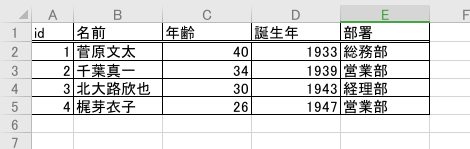
\includegraphics[width=10cm]{img/table03.png}
\vspace{3mm}

primary key には、数字やコードが使われる。
\footnote{'001'や'C001'など、固定長の文字列がよく使われる。また、整数もよく使われる。可変長の文字列は使われない。正確さに欠ける。}


\section{データベースを作成する}

\subsection{データベースの作成}

''rensyu'' というデータベースを作成する。

\begin{tcolorbox}
 mysql$>$ create database rensyu \ $<$Enterキー$>$
\end{tcolorbox}

このように入力すると、以下のようになる。

\begin{tcolorbox}
 mysql$>$ create database rensyu \\
     -$>$ 
\end{tcolorbox}

これは、入力の終わりがまだないので、次の入力を受け付けているのである。

入力の終わりは ``;''(セミコロン) あるいは ``\textbackslash g'' である。
 
\begin{tcolorbox}
 mysql$>$ create database rensyu \\
     -$>$ ;  \ $<$Enterキー$>$
\end{tcolorbox}

``;''(セミコロン) あるいは ''\textbackslash g'' を入力して <Enterキー>
を押す。

\subsection{データベースの確認}

データベースがちゃんと作成できたか、確認する。

\begin{tcolorbox}
 mysql$>$ show databases; \hspace{3mm} (複数形)
\end{tcolorbox}

\begin{lstlisting}[numbers=none]
+--------------------+
| Database           |
+--------------------+
| information_schema |
| rensyu             |
+--------------------+
\end{lstlisting}


\subsection{データベースの使用宣言}

まず、使用宣言を行う。

\begin{tcolorbox}
 mysql$>$ use rensyu;
\end{tcolorbox}

\fbox{Database changed} と表示される。



\end{document}

%% 修正時刻: Sat May  2 15:10:04 2020


%% 修正時刻: Sat 2022/10/01 08:45:160
